\documentclass[border=1mm]{standalone}
\usepackage[T1]{fontenc}
\usepackage[scaled=0.92]{helvet}
\renewcommand\familydefault{\sfdefault}
\usepackage{amssymb}
\usepackage{tikz}
\usetikzlibrary{arrows.meta,calc,shapes.geometric}
% ---- shared style (methodology figures) ----
\definecolor{mA}{HTML}{1B7F79}\definecolor{mAl}{HTML}{E4F2F0}
\definecolor{mB}{HTML}{2F5F98}\definecolor{mBl}{HTML}{E7EEF7}
\definecolor{mC}{HTML}{B85A16}\definecolor{mCl}{HTML}{FBEEDF}
\definecolor{ink}{HTML}{262626}\definecolor{mute}{HTML}{6B6B6B}
\definecolor{grey}{HTML}{8C8C8C}\definecolor{greyl}{HTML}{EFEFEF}
% pathway colours: ECM, TGF-beta, stellate, inflammation, apoptosis/stress, hepatocyte
\definecolor{pw0}{HTML}{B85A16}\definecolor{pw1}{HTML}{D9A21B}\definecolor{pw2}{HTML}{8A5BA6}
\definecolor{pw3}{HTML}{C2413B}\definecolor{pw4}{HTML}{6E8B3D}\definecolor{pw5}{HTML}{2F5F98}
\newcommand\fs{\fontsize{7}{8.4}\selectfont}
\newcommand\fss{\fontsize{6.3}{7.5}\selectfont}
\newcommand\fsx{\fontsize{5.8}{6.8}\selectfont}
\newcommand\fsh{\fontsize{7.6}{9}\selectfont\bfseries}
\newcommand\fsn{\fontsize{9}{10}\selectfont\bfseries}
\hyphenpenalty=10000 \exhyphenpenalty=10000
\tikzset{
  >={Stealth[length=2mm,width=1.6mm]},
  flow/.style={->,line width=0.8pt,draw=ink!70},
  thin/.style={->,line width=0.5pt,draw=ink!60},
  gedge/.style={draw=black!22,line width=0.25pt},
  gnode/.style={circle,draw=white,line width=0.25pt,inner sep=0pt,minimum size=1.45mm},
  ttl/.style={anchor=west,font=\fsh},
}
% cylinder: \cyl{colour}{x centre}{base y}{height}{width}
\newcommand\cyl[5]{%
  \filldraw[fill=#1!35,draw=#1,line width=0.5pt] ({#2-#5/2},{#3+#4}) -- ({#2-#5/2},#3) arc[start angle=180,end angle=360,x radius=#5/2,y radius=0.9] -- ({#2+#5/2},{#3+#4});
  \filldraw[fill=#1!12,draw=#1,line width=0.5pt] (#2,{#3+#4}) ellipse[x radius=#5/2,y radius=0.9];}
% numbered module badge
\newcommand\badge[3]{\node[circle,fill=#1,text=white,inner sep=0pt,minimum size=4.6mm,font=\fss\bfseries] at #2 {#3};}
\begin{document}
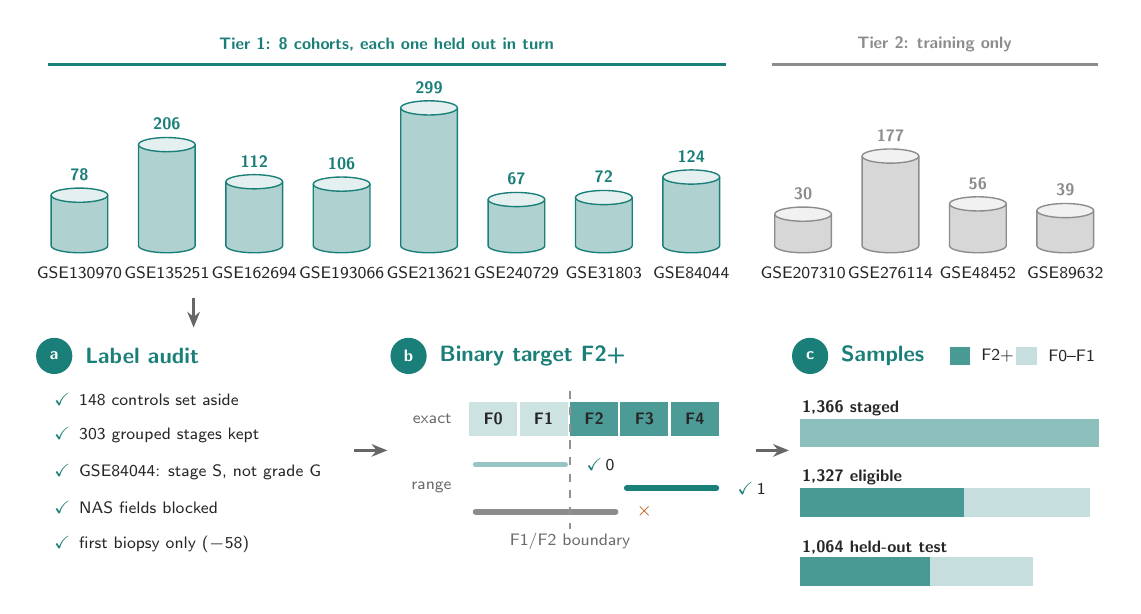
\begin{tikzpicture}[x=1mm,y=1mm,font=\fs,text=ink]
% ---------------- cohorts: cylinder height proportional to n ----------------
\foreach \acc/\n [count=\i from 0] in {GSE130970/78,GSE135251/206,GSE162694/112,GSE193066/106,GSE213621/299,GSE240729/67,GSE31803/72,GSE84044/124}{
  \pgfmathsetmacro\h{2.5+\n/299*15}
  \pgfmathsetmacro\x{5.5+\i*11.1}
  \cyl{mA}{\x}{46}{\h}{7.2}
  \node[font=\fss\bfseries,text=mA] at (\x,{46+\h+2.6}) {\n};
  \node[font=\fsx] at (\x,42.6) {\acc};}
\foreach \acc/\n [count=\i from 0] in {GSE207310/30,GSE276114/177,GSE48452/56,GSE89632/39}{
  \pgfmathsetmacro\h{2.5+\n/299*15}
  \pgfmathsetmacro\x{97.4+\i*11.1}
  \cyl{grey}{\x}{46}{\h}{7.2}
  \node[font=\fss\bfseries,text=grey] at (\x,{46+\h+2.6}) {\n};
  \node[font=\fsx] at (\x,42.6) {\acc};}
\draw[mA,line width=0.8pt] (1.5,69) -- (87.6,69);
\node[anchor=south,font=\fss\bfseries,text=mA] at (44.5,69.4) {Tier 1: 8 cohorts, each one held out in turn};
\draw[grey,line width=0.8pt] (93.4,69) -- (134.8,69);
\node[anchor=south,font=\fss\bfseries,text=grey] at (114.1,69.4) {Tier 2: training only};
% ---------------- row 2 ----------------
\draw[flow] (20,39.4)--(20,35.6);
% (a) label audit
\badge{mA}{(2.3,32)}{a}
\node[ttl,text=mA] at (5,32) {Label audit};
\newcommand\chk[2]{\node[anchor=west,font=\fss] at (1,#1) {\textcolor{mA}{\checkmark}\, #2};}
\chk{26.5}{148 controls set aside}
\chk{21.9}{303 grouped stages kept}
\chk{17.3}{GSE84044: stage S, not grade G}
\chk{12.7}{NAS fields blocked}
\chk{8.1}{first biopsy only ($-$58)}
\draw[flow] (40.4,20)--(44.6,20);
% (b) F2+ rule on the stage scale
\badge{mA}{(47.3,32)}{b}
\node[ttl,text=mA] at (50,32) {Binary target F2+};
\foreach \s [count=\i from 0] in {F0,F1,F2,F3,F4}{
  \ifnum\i<2 \def\cellc{mA!22}\else\def\cellc{mA!78}\fi
  \fill[\cellc] (55+\i*6.4,21.8) rectangle ++(6.1,4.4);
  \node[font=\fss\bfseries,text=ink] at (58.05+\i*6.4,24) {\s};}
\newcommand\grp[5]{% x0 x1 y colour mark
  \draw[#4,line width=2pt,line cap=round] (#1,#3)--(#2,#3);
  \node[anchor=west,font=\fss] at (#2+1.4,#3) {#5};}
\node[anchor=east,font=\fsx,text=mute] at (54,24) {exact};
\node[anchor=east,font=\fsx,text=mute] at (54,15.3) {range};
\grp{55.8}{67.2}{18.2}{mA!45}{\textcolor{mA}{\checkmark}\,0}
\grp{75.0}{86.4}{15.2}{mA}{\textcolor{mA}{\checkmark}\,1}
\grp{55.8}{73.6}{12.2}{grey}{\textcolor{mC}{$\times$}}
\draw[ink!50,dashed,line width=0.5pt] (67.8,27.6)--(67.8,10);
\node[font=\fsx,text=mute] at (67.8,8.4) {F1/F2 boundary};
\draw[flow] (91.4,20)--(95.6,20);
% (c) sample funnel, bars to scale
\badge{mA}{(98.3,32)}{c}
\node[ttl,text=mA] at (101,32) {Samples};
\newcommand\sbar[6]{% y, total width, pos width, label, pos label, neg label
  \fill[mA!80] (97,#1) rectangle ++(#3,3.6);
  \fill[mA!25] (97+#3,#1) rectangle ++(#2-#3,3.6);
  \node[anchor=south west,font=\fss\bfseries,inner sep=0.6pt] at (97,#1+3.7) {#4};}
\fill[mA!50] (97,20.4) rectangle ++(38,3.6);
\node[anchor=south west,font=\fss\bfseries,inner sep=0.6pt] at (97,24.1) {1,366 staged};
\sbar{11.6}{36.9}{20.9}{1,327 eligible}{}{}
\sbar{2.8}{29.6}{16.5}{1,064 held-out test}{}{}
\fill[mA!80] (116,30.9) rectangle ++(2.6,2.2); \node[anchor=west,font=\fsx] at (118.8,32) {F2+};
\fill[mA!25] (124.5,30.9) rectangle ++(2.6,2.2); \node[anchor=west,font=\fsx] at (127.3,32) {F0--F1};
\end{tikzpicture}
\end{document}
